\documentclass[11pt]{standalone}
\usepackage{amssymb}
\usepackage{amsmath}
\usepackage[no-math]{fontspec}
\usepackage{unicode-math}
\setmainfont{Libertinus Sans}
\setsansfont{Libertinus Sans}
\setmathfont{Libertinus Math}
\usepackage{pgf,xcolor}
\usepackage{tikz}
\usetikzlibrary{arrows.meta, backgrounds, calc}
\usepackage{pgfplots}
\pgfplotsset{compat=newest}

\definecolor{my_darkgray}{HTML}{484949}
\definecolor{my_lightgray}{HTML}{F3F4F4}
\definecolor{my_darkblue}{HTML}{005A94}
\definecolor{my_lightblue}{HTML}{CCDEE9}
\definecolor{my_yellow}{HTML}{FFEC7F}
\definecolor{my_red}{HTML}{E60000}
\definecolor{my_orange}{HTML}{E87846}

\begin{document}
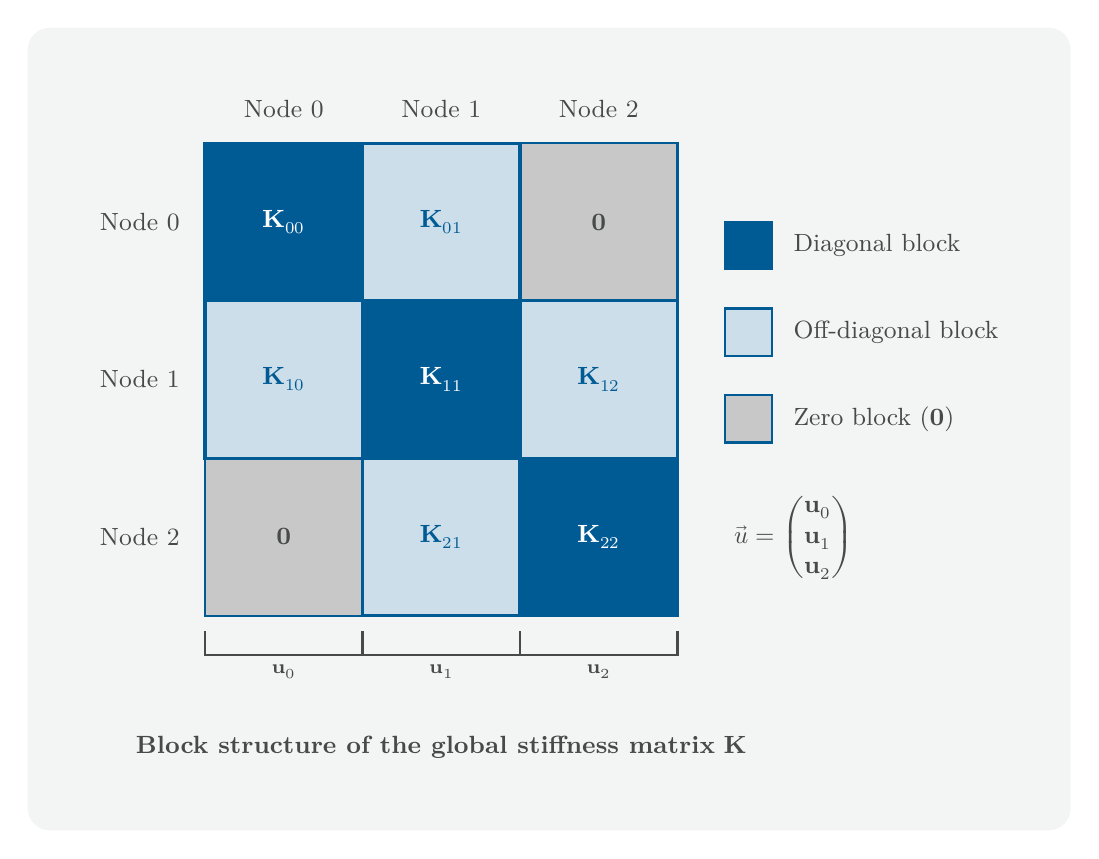
\begin{tikzpicture}[
    show background rectangle,
    background rectangle/.style={fill=my_lightgray, rounded corners=8pt},
    inner frame sep=0.8cm
]

    %------------------------------------------------------------
    % Nullblöcke grau hinterlegen (K_02, K_20)
    %------------------------------------------------------------
    \filldraw[fill=my_darkgray!30, draw=none]
        (4,0) rectangle (6,-2);
    \filldraw[fill=my_darkgray!30, draw=none]
        (0,-4) rectangle (2,-6);

    %------------------------------------------------------------
    % Besetzte Nebendiagonalblöcke hellblau hinterlegen
    % (K_01, K_10, K_12, K_21)
    %------------------------------------------------------------
    \foreach \x/\y in {3/-1, 1/-3, 5/-3, 3/-5} {
        \filldraw[fill=my_lightblue, draw=my_darkblue, very thick]
            (\x-1,\y+1) rectangle (\x+1,\y-1);
    }

    %------------------------------------------------------------
    % Diagonalblöcke dunkelblau hinterlegen (K_00, K_11, K_22)
    %------------------------------------------------------------
    \foreach \x/\y in {1/-1, 3/-3, 5/-5} {
        \filldraw[fill=my_darkblue, draw=my_darkblue, very thick]
            (\x-1,\y+1) rectangle (\x+1,\y-1);
    }

    %------------------------------------------------------------
    % Rahmen und Blockgrenzen
    %------------------------------------------------------------
    \draw[draw=my_darkblue, thick] (0,0) rectangle (6,-6);
    \draw[draw=my_darkblue, thick] (2,0)  -- (2,-6);
    \draw[draw=my_darkblue, thick] (4,0)  -- (4,-6);
    \draw[draw=my_darkblue, thick] (0,-2) -- (6,-2);
    \draw[draw=my_darkblue, thick] (0,-4) -- (6,-4);

    %------------------------------------------------------------
    % Block-Labels
    %------------------------------------------------------------
    % Diagonalblöcke (weiße Schrift)
    \node[font=\small, text=white] at (1,-1) {$\mathbf{K}_{00}$};
    \node[font=\small, text=white] at (3,-3) {$\mathbf{K}_{11}$};
    \node[font=\small, text=white] at (5,-5) {$\mathbf{K}_{22}$};

    % Besetzte Nebendiagonalblöcke (dunkelblaue Schrift)
    \node[font=\small, text=my_darkblue] at (3,-1) {$\mathbf{K}_{01}$};
    \node[font=\small, text=my_darkblue] at (1,-3) {$\mathbf{K}_{10}$};
    \node[font=\small, text=my_darkblue] at (5,-3) {$\mathbf{K}_{12}$};
    \node[font=\small, text=my_darkblue] at (3,-5) {$\mathbf{K}_{21}$};

    % Nullblöcke (grau)
    \node[font=\small, text=my_darkgray] at (5,-1) {$\mathbf{0}$};
    \node[font=\small, text=my_darkgray] at (1,-5) {$\mathbf{0}$};

    %------------------------------------------------------------
    % Knotenlabels an den Rändern
    %------------------------------------------------------------
    \node[font=\small, text=my_darkgray, anchor=east]  at (-0.2,-1) {Node 0};
    \node[font=\small, text=my_darkgray, anchor=east]  at (-0.2,-3) {Node 1};
    \node[font=\small, text=my_darkgray, anchor=east]  at (-0.2,-5) {Node 2};

    \node[font=\small, text=my_darkgray, anchor=south] at (1, 0.2) {Node 0};
    \node[font=\small, text=my_darkgray, anchor=south] at (3, 0.2) {Node 1};
    \node[font=\small, text=my_darkgray, anchor=south] at (5, 0.2) {Node 2};

    %------------------------------------------------------------
    % Klammern unten: Spaltengruppierung u0, u1, u2
    %------------------------------------------------------------
    \draw[draw=my_darkgray, thick]
        (0.0,-6.2) -- (0.0,-6.5) -- (2.0,-6.5) -- (2.0,-6.2);
    \draw[draw=my_darkgray, thick]
        (2.0,-6.2) -- (2.0,-6.5) -- (4.0,-6.5) -- (4.0,-6.2);
    \draw[draw=my_darkgray, thick]
        (4.0,-6.2) -- (4.0,-6.5) -- (6.0,-6.5) -- (6.0,-6.2);

    \node[font=\scriptsize, text=my_darkgray, anchor=north] at (1.0,-6.5)
        {$\mathbf{u}_0$};
    \node[font=\scriptsize, text=my_darkgray, anchor=north] at (3.0,-6.5)
        {$\mathbf{u}_1$};
    \node[font=\scriptsize, text=my_darkgray, anchor=north] at (5.0,-6.5)
        {$\mathbf{u}_2$};

    %------------------------------------------------------------
    % Legende
    %------------------------------------------------------------
    \filldraw[fill=my_darkblue, draw=my_darkblue, thick]
        (6.6,-1.0) rectangle (7.2,-1.6);
    \node[font=\small, text=my_darkgray, anchor=west] at (7.35,-1.3)
        {Diagonal block};

    \filldraw[fill=my_lightblue, draw=my_darkblue, thick]
        (6.6,-2.1) rectangle (7.2,-2.7);
    \node[font=\small, text=my_darkgray, anchor=west] at (7.35,-2.4)
        {Off-diagonal block};

    \filldraw[fill=my_darkgray!30, draw=my_darkblue, thick]
        (6.6,-3.2) rectangle (7.2,-3.8);
    \node[font=\small, text=my_darkgray, anchor=west] at (7.35,-3.5)
        {Zero block ($\mathbf{0}$)};

    %------------------------------------------------------------
    % Verschiebungsvektor rechts
    %------------------------------------------------------------
    \node[font=\small, text=my_darkgray, anchor=west] at (6.6,-5.0)
        {$\vec{u} =
        \begin{pmatrix}
        \mathbf{u}_0 \\ \mathbf{u}_1 \\ \mathbf{u}_2
        \end{pmatrix}$};

    %------------------------------------------------------------
    % Titel
    %------------------------------------------------------------
    \node[font=\small, text=my_darkgray, anchor=north]
        at (3,-7.4)
        {\textbf{Block structure of the global stiffness matrix} $\mathbf{K}$};

\end{tikzpicture}
\end{document}